\documentclass{article}
\usepackage[utf8]{inputenc}
\usepackage{amsmath,amssymb,amsthm}
\usepackage{graphicx}
\usepackage{floatrow}
\usepackage{blindtext}
\usepackage[T1]{fontenc}
\usepackage[font=small,labelfont=bf,tableposition=top]{caption}
\usepackage[export]{adjustbox}

\DeclareCaptionLabelFormat{andtable}{#1~#2  \&  \tablename~\thetable}

\newcommand{\stirlingone}[2]{\begin{bmatrix} #1\\#2 \end{bmatrix}}
\newcommand{\stirlingtwo}[2]{\begin{Bmatrix} #1\\#2 \end{Bmatrix}}

\newtheorem{definition}{Definition}[subsection]
\newtheorem{question}[definition]{Question to Ponder}
\newtheorem{theorem}[definition]{Theorem}
\newtheorem{lemma}[definition]{Lemma}
\newtheorem{remark}[definition]{Remark}
\newtheorem{example}[definition]{Example}
\newtheorem{exercise}[definition]{Exercise}
\newtheorem{corollary}[definition]{Corollary}
\newtheorem{proposition}[definition]{Proposition}

\title{Combinatorics Final Project: \\ The Max-Cut Problem}
\author{Evan Wagner}
\date{April 2022}

\begin{document}

\maketitle

\vspace{1in}

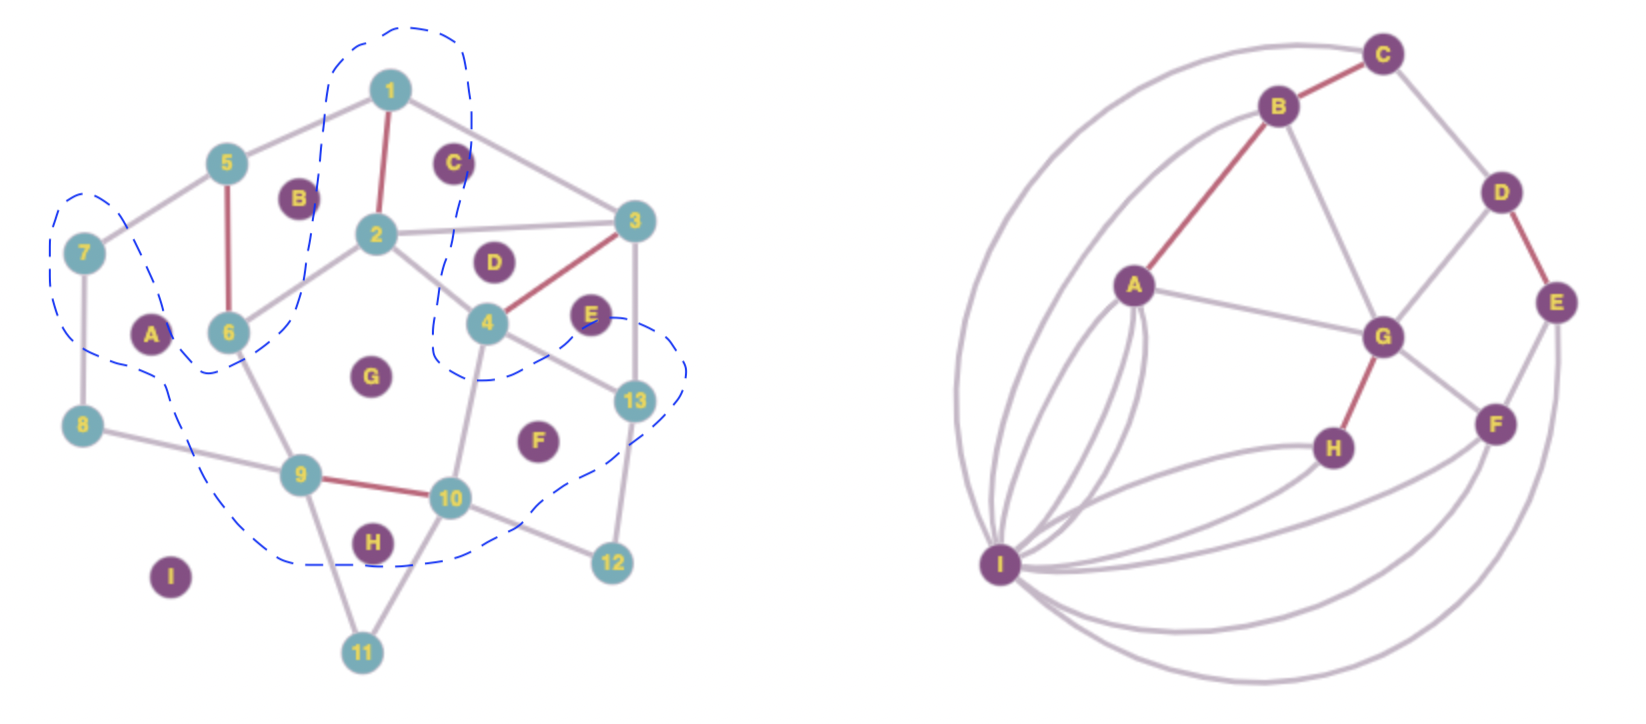
\includegraphics[scale=.5, center]{planar_dual_cut.png}


\section{Introduction}

\par Given a graph with weighted edges, partition its vertices into two groups such that the sum of the weights of all the edges incident to both parts is maximized. This problem is known as the \textit{max-cut problem}, or \textit{weighted max-cut problem}. In 1972, Richard Karp showed that this problem is $NP$-complete, which means a computer can easily verify a proposed solution to the problem, but there is no computationally efficient way to find a solution in the first place.\cite{Karp} Karp's paper kicked off a wide search for bounds, approximations, and other mathematical truths about the max-cut problem. \\

\par Large graphs are very useful models for analyzing complex systems, such as natural phenomena, social relationships, mechanical devices, and the like.  Solutions to max-cut and similar problems have important implications in many subject areas, including network architecture, molecular structure, and forest management. \\

\par Today, the rapid proliferation of deep neural networks (DNNs) presents new uses for combinatorial optimization. The complexity of DNN architecture often obscures how the models arrive at their conclusions based on the data they are fed. Considering DNNs as large weighted directional graphs, finding heavily-weighted structures within them using problems like max-cut may help researchers to unlock the secrets of their creations. \\

\subsection{The Problem Spaces $P$ and $NP$}

\par Karp's paper popularized a characterization of problems based on whether a computer can solve them in a pre-determinable amount of time.\cite{Karp} We say a problem $Q$ is in $P$ if and only if there exists an algorithm that is guaranteed to solve $Q$ in a running time bounded above by $O(n^k)$, where $n$ measures the size of the input and $k$ is some known constant. Any problem that can be reduced\footnote{A reduction of a problem turns it into another problem that is satisfied by the same input.} in polynomial time to a $P$-complete problem is itself $P$-complete. Much research is devoted to finding such transformations. \\

\par In contrast, a problem $Q$ is in $NP$ if it cannot be solved in polynomial time by deterministic algorithms. However, any guess of a solution to $Q$ can be verified to be correct or incorrect in polynomial time.\footnote{We know that $P \subseteq NP$ because for any problem that can be solved in polynomial time, its solution can also be verified in polynomial time. Interestingly, whether $P = NP$ has not been proved nor disproved. The field of cryptography is based entirely on the assumption that $P \not= NP$, so proving that $P = NP$ could destroy much of the protective architecture of the digital sphere.} If a problem $Q$ can be reduced to any problem in $NP$, we call it $NP$-hard. If that problem is also in $NP$ itself, we call it $NP$-complete. The general max-cut problem is $NP$-complete, but has been shown to be $P$-complete for specific graph types.

\section{The Max-Cut Problem}

\begin{figure}[h]
    \centering
    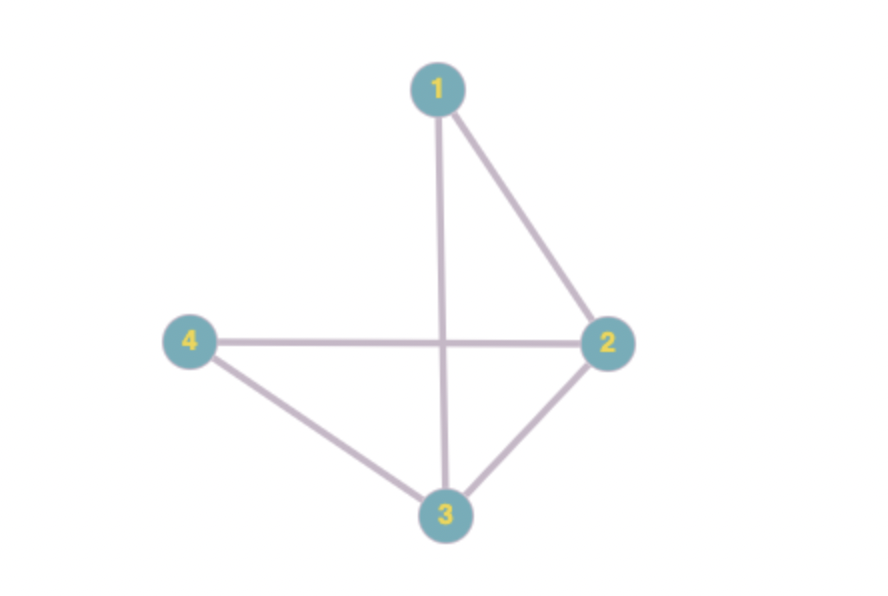
\includegraphics[scale=.35]{four_vertex.png}
    \caption{A 4-vertex graph $G$}
    \label{fig:four_vertex}
\end{figure}

\par Let $G$ be a graph with vertices $\{v_1,v_2,\dots,v_n\}$. To make a cut $\{S,\bar{S}\}$, we choose a subset of vertices $S$ such that both $S$ and its complement $\bar{S}$ are non-empty. There are $\stirlingtwo{n}{2}$ ways to do this. As $n$ increases, the increase in complexity of the problem accelerates greatly in what computer scientists often call a \textit{combinatorial explosion}. That is why the max-cut problem is $NP$-hard. \\

\par In the weighted version of max cut, a weight function $w(e_i)$ or $w(v_i,v_j)$ assigns a constant to each edge given by the vertex pair $v_i,v_j$ where $1\le i<j\le |V|$. Weights are more conveniently notated $w_{ij}$. They are often between 0 and 1, or non-negative at least. Vertex pairs with no edge are set to 0. For simplicity, we can think of an unweighted graph as a weighted graph with weights in $\{0,1\}$. The weight of a cut is the sum of the weights of the edges in it. In other terms, $w(S,\bar{S}) = \sum_{e\in (S,\bar{S})} w(e)$. \\

\par Now, for each vertex $v_i$, define the following:

$$y_i := \begin{cases}
    1 \quad &\text{if} \,\, v_i\in S \\
    -1 \quad &\text{otherwise.} \\
\end{cases}$$

\par It follows that the weight of the cut $(S, \bar{S})$ is given by $$w(S,\bar{S}) = \frac{1}{2}\sum_{i<j}  w_{ij}(1-y_iy_j).\footnote{If $v_i$ and $v_j$ are both in $S$ or $\bar{S}$, the corresponding term in this sum is 0. If, on the other hand, $v_i$ and $v_j$ are in different sets, the term contributes $w_{ij}$ to the sum. So the sum adds up the weights of only the edges that cross the cut.}$$ The edges whose weights maximize this function are the maximum cut of $G$. \\

\subsection{Example: Max Cut of a 4-Vertex Graph}

\par Consider the graph shown in Figure \ref{fig:four_vertex}. It has 4 vertices and thus only $\stirlingtwo{4}{2} = 7$ possible cuts, so we can easily check each one to see which contains the most edges. Table 1 gives the number of edges in each cut, which the reader can verify visually. The maximum cut, shown in Figure \ref{fig:four_vertex_cut}, separates vertices 1 and 4 from 2 and 3 and crosses a total of 4 edges. \\

\begin{figure}[!ht]
    \centering
    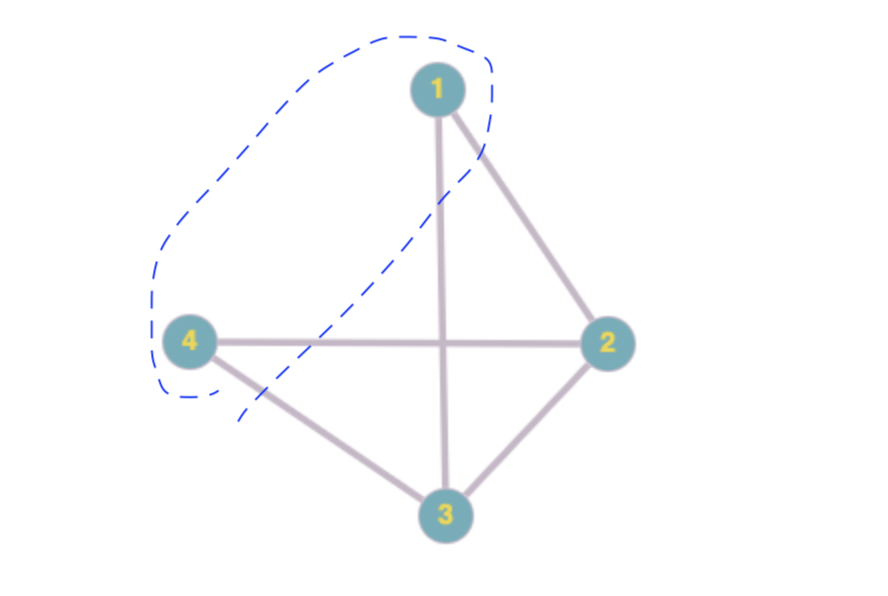
\includegraphics[scale=.35]{four_vertex_cut.png}
    \qquad
    \begin{tabular}[b]{|c|c|}
        \hline
        Cut & Size \\
        \hline
        $\{1,234\}$ & 2\\
        $\{2,134\}$ & 3\\
        $\{3,124\}$ & 3\\
        $\{4,123\}$ & 2\\
        $\{12,34\}$ & 3\\
        $\{13,24\}$ & 3\\
        $\{14,23\}$ & 4\\
        \hline
    \end{tabular}
    \captionlistentry[table]{A table beside a figure}
    \captionsetup{labelformat=andtable}
    \caption{The maximum cut of $G$}
    \label{fig:four_vertex_cut}
\end{figure}

\par What if we assign weights $w_{ij}$ to each edge, as shown in Figure \ref{fig:four_vertex_weighted_cut}? The maximum cut for this weighted graph is now $\{12,34\}$. Though it crosses fewer edges than $\{14,23\}$, its total weight is highest because its edges have relatively high individual weight compared to the rest. \\

\begin{figure}[!ht]
    \centering
    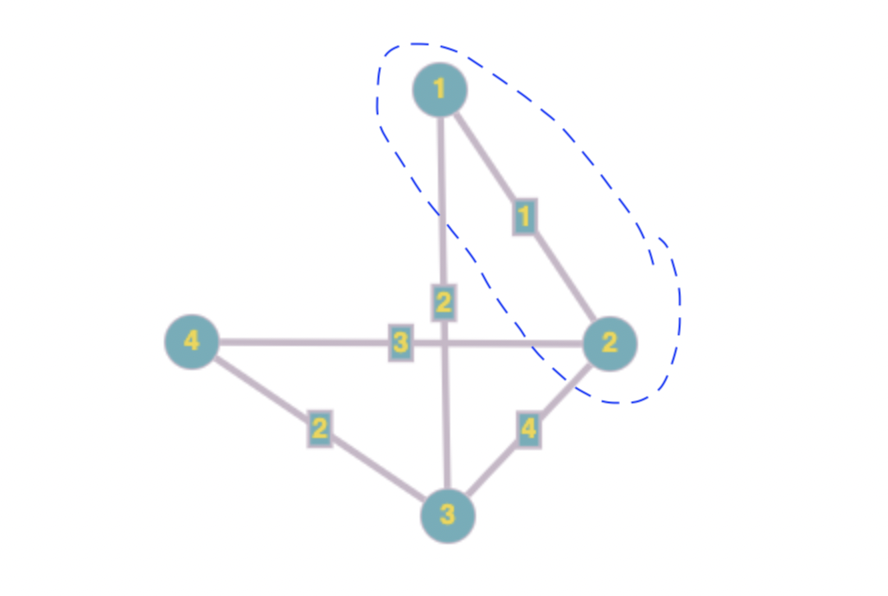
\includegraphics[scale=.35]{four_vertex_weighted_cut.png}
    \qquad
    \begin{tabular}[b]{|c|c|}
        \hline
        Cut & Size \\
        \hline
        $\{1,234\}$ & 3 \\
        $\{2,134\}$ & 8 \\
        $\{3,124\}$ & 8 \\
        $\{4,123\}$ & 5 \\
        $\{12,34\}$ & 9 \\
        $\{13,24\}$ & 7 \\
        $\{14,23\}$ & 8 \\
        \hline
    \end{tabular}
    \captionlistentry[table]{A table beside a figure}
    \captionsetup{labelformat=andtable}
    \caption{The maximum cut of weighted $G$}
    \label{fig:four_vertex_weighted_cut}
\end{figure}

\newpage

\subsection{Reformulating the Weight Function in Matrix Notation}

\par We can frame the problem in the language of linear algebra to more easily compute the weight of a given cut. Define the weight matrix $W := [w_{ij}]_{1 \le i \le n, 1 \le j \le n}$, and a cut as a binary vector $x$ of length $n$, where the $k$-th entry of $x$ is 1 if $v_k\in S$, 0 otherwise. Then the weight of the cut $x$ is given by $f(x) = x^T W(u-x)$, where $u$ is the length-$n$ vector of 1s. \\

\par We may now use a simple MATLAB program to compute the weight of a cut, shown in Figure \ref{fig:matlab_cut_weight_function}. \\

\begin{figure}[h]
    \centering
    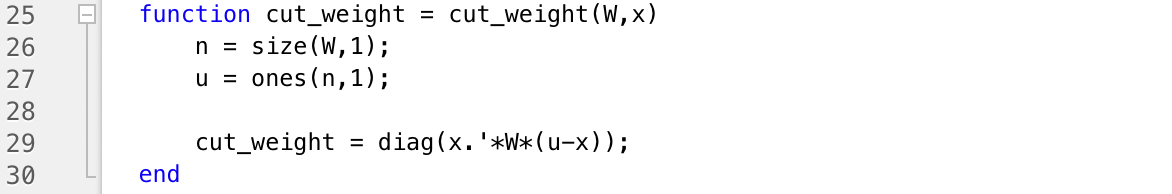
\includegraphics[scale=.5]{matlab_function.png}
    \caption{A MATLAB function that computes the weight of a cut $x$ given a weight matrix $W$}
    \label{fig:matlab_cut_weight_function}
\end{figure}

\par To save time, we can test multiple cuts at once by setting $x$ as a matrix with each column a cut. Then the $i$th entry of the output vector is the weight of the cut given by the $i$th column of $W$. Testing the function on our example above, Figure \ref{fig:matlab_four_vertex} shows that it returns the same answers we found earlier. \\

\begin{figure}[h]
    \centering 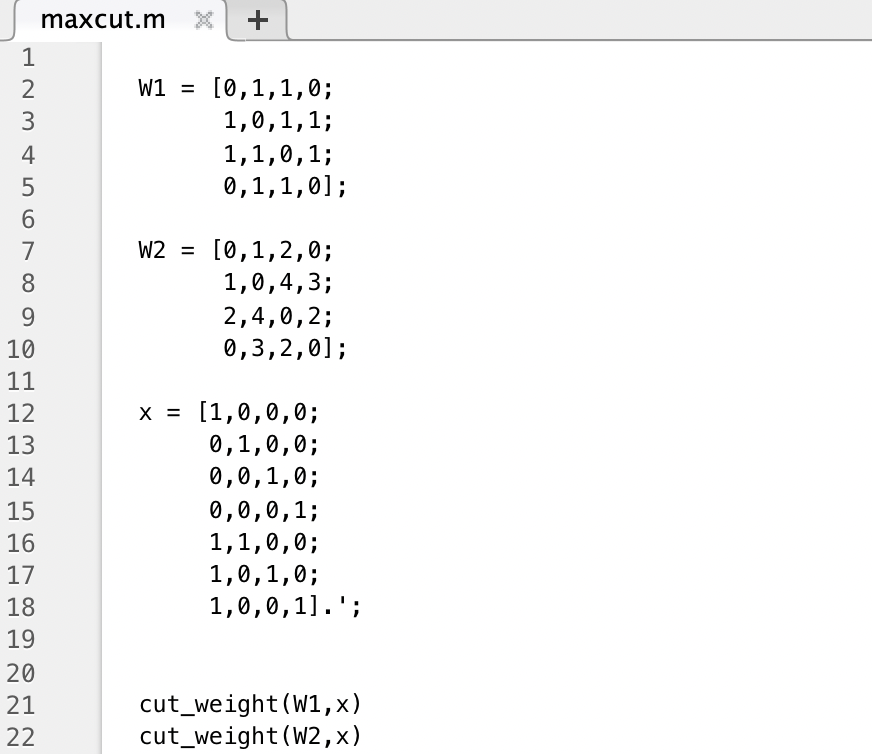
\includegraphics[scale=.5]{matlab_program.png}
    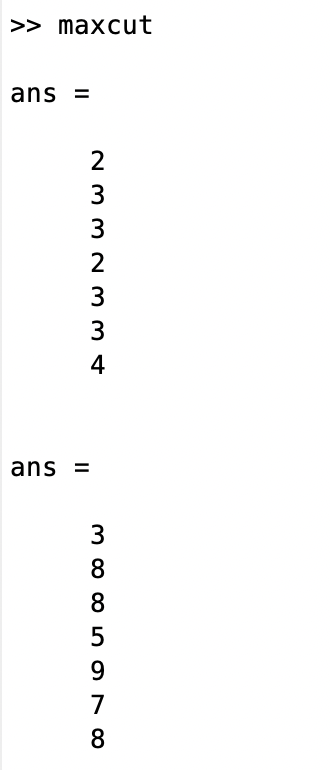
\includegraphics[scale=.5]{matlab_output.png}
    \caption{Computing the cuts from Example 2.1 with MATLAB}
    \label{fig:matlab_four_vertex}
\end{figure}



\section{P-Solution: Max-Cut on Planar Graphs}

\par In 1974, F. Hadlock proved that the maximum cut of a \textit{planar graph} is equivalent to another problem with a known polynomial time algorithm.\cite{Hadlock} A graph is planar if it can be embedded in a plane such that none of its edges cross. Hadlock's result has many practical applications. All forests are planar graphs, as are most geographic maps, many chemical bond charts, and more. I will prove Hadlock's claim, following the same broad steps but using my own arguments.

\begin{figure}[h]
    \centering
    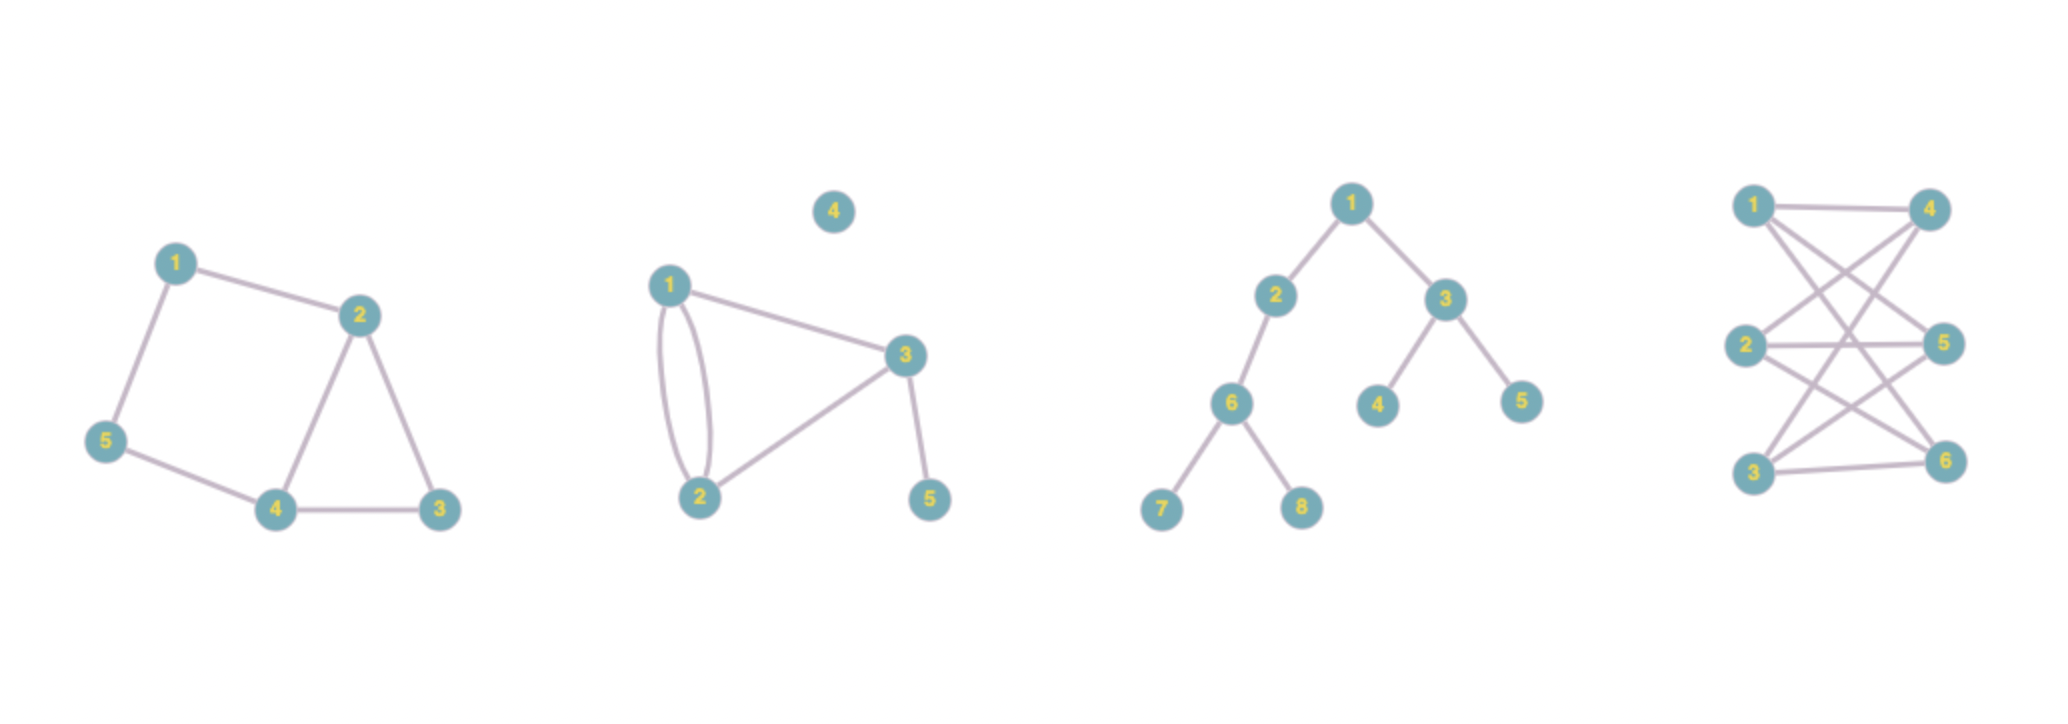
\includegraphics[scale=.35]{planar_examples.png}
    \caption{All of these graphs are planar except the rightmost graph, $K_{3,3}$, whose edges cannot all avoid crossing each other}
    \label{fig:planar_examples}
\end{figure}

\par First, we state some definitions. Given a graph $G$, a \textit{circuit} is a sequence of $m$ distinct edges $\{x_0,x_1\},\{x_1,x_2\},\dots,\{x_{m-1},x_0\}$. The length of a circuit is the number of edges in it. Now consider a subset of the graph's edges $F$. $F$ is an \textit{odd-circuit cover} for $G$ if the graph $G'$ formed by removing $F$ from $G$ has no circuits of odd length. $F$ is an \textit{odd-vertex pairing} if it connects each pair of odd vertices by exactly one path. \\

\begin{lemma}
    The complement of a maximum cut of a graph $G$ is a minimum odd-circuit cover for $G$.\cite{Hadlock}
    \label{lem:max-cut-min-odd-circ}
\end{lemma}

\begin{proof}
    First we will prove that any cut of $G$ is an odd-circuit cover for $G$. Let the set of edges $(S,\bar{S})$ represent a cut of a graph $G$, and let $F_{\alpha}$ be a circuit in $G$. If all vertices in the edges of $F_{\alpha}$ are in the same subset (either $S$ or $\bar{S}$), then $|F_{\alpha} \cap (S,\bar{S})| = 0$, which is even. If we switch one of the vertices to the other side of the cut, its two adjacent edges in $F_{\alpha}$ are either added to or removed from $(S,\bar{S})$, so $|F_{\alpha} \cap (S,\bar{S})|$ will always be even. It follows that any odd circuit in $G$ must have at least one edge outside of the cut. Therefore, the complement of $F_{\alpha}$ is an odd-circuit cover. \\
    
\newpage
    
    For the other direction, consider an arbitrary odd-circuit cover $F_{\beta}$ in $G$. Then its complement $F_{\beta}^{\mathcal{C}}$ contains only even circuits, and therefore only even cycles.\footnote{Cycles are circuits with distinct vertices. Any circuit is made up of one or more cycles, and any cycle is itself a circuit.} By Shahriari's Theorem 10.37,\cite{Shahriari} $E_{OC}^{\mathcal{C}}$ forms a bipartite graph, so all of its edges can be contained in a single cut. \\
    
    We have now proved that any cut of $G$ is an odd-circuit cover for $G$. To prove the original claim, we simply observe that if the sum of weights on a cut is the greatest possible, then the sum of weights on its complement is the least possible.
\end{proof}

\par Here is where planar graphs come in: they have a unique \textit{geometric dual}. Embedding $G$ in a plane partitions it into $k$ faces, and the geometric dual $G_d$ of $G$ has $k$ vertices which each correspond to one of the $k$ faces. For each edge in $G$ that is adjacent to the parts $\alpha$ and $\beta$, the two vertices $v_{\alpha},v_{\beta} \in G_d$ are connected by an edge. The weight of the edge in $G_d$ is the weight of the corresponding edge in $G$.\footnote{Geometric duals can be hard to conceptualize just from reading about them. The example in Section 3.1 should give the reader a more intuitive walkthrough of the process of finding a geometric dual.} \\

\begin{figure}[h]
    \centering
    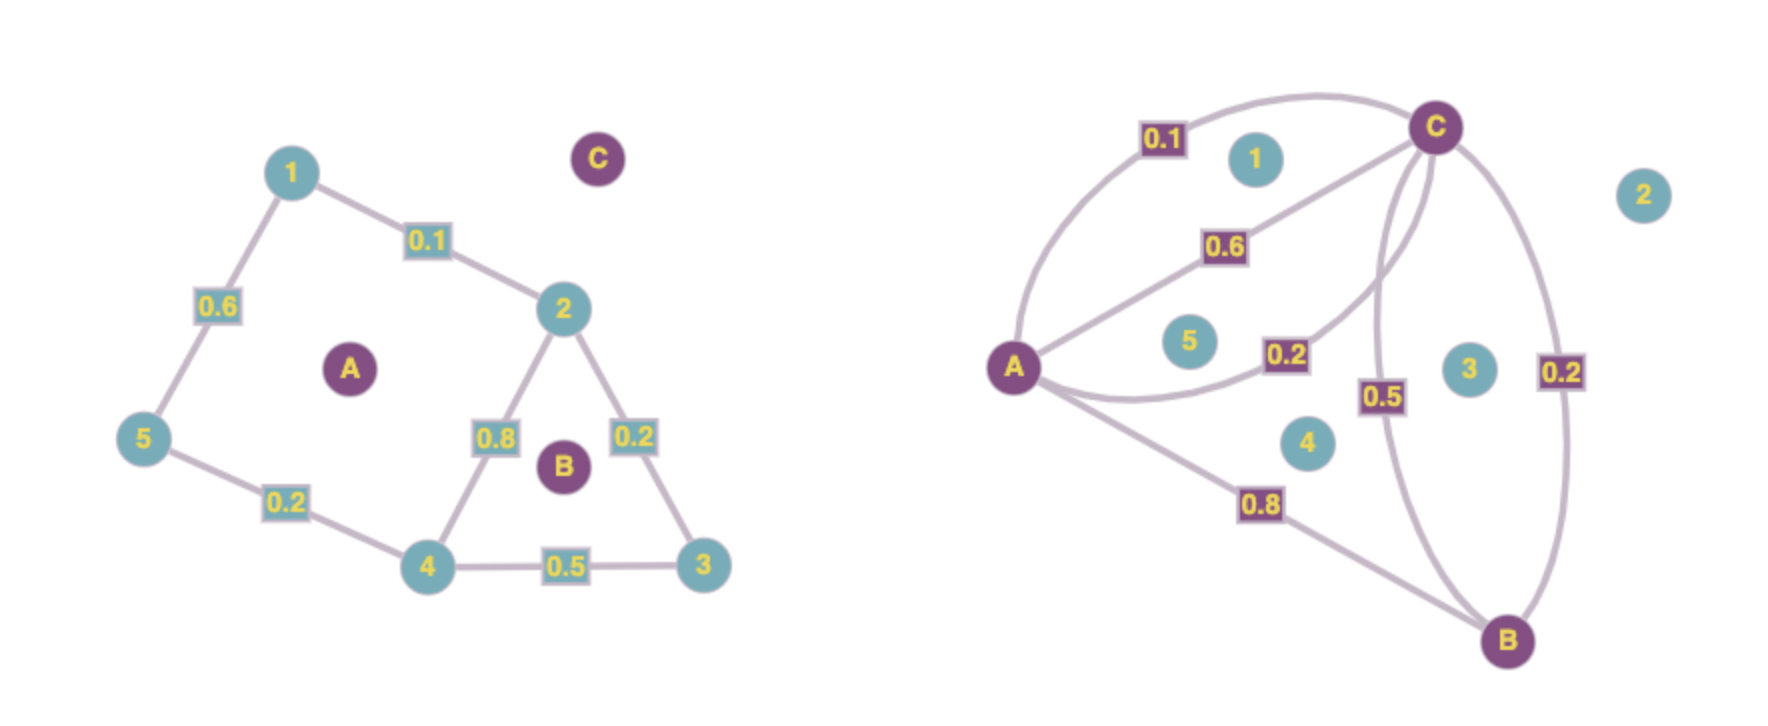
\includegraphics[scale=.35]{geom_dual.png}
    \caption{A planar graph $G$ and its geometric dual $G_d$.}
    \label{fig:geom_dual}
\end{figure}

\par Not only is $G_d$ unique for each embedding of any planar graph $G$, but its geometric dual $(G_d)_d = G$.\cite{hadlock} The reader can visually confirm an example of this in Figure \ref{fig:geom_dual}. Then each subset of edges in $G_d$ is related to exactly one in $G$ that can be found by taking a geometric dual. We take advantage of this fact to find an optimal structure in $G_d$ that corresponds to the minimum odd-circuit cover of Lemma \ref{lem:max-cut-min-odd-circ}.

\newpage

\begin{theorem}
    The maximum cut of a graph $G$ corresponds to the minimum odd-vertex pairing of $G_d$.\cite{Hadlock}
\end{theorem}

\begin{proof}
    Since $\sum_{i=1}^{n} \text{deg}(v_i) = 2|E|$ for any graph, the number of odd-degree vertices in $G$ must be even, so they can be paired off with none left over. An odd-vertex pairing connects each pair of odd-degree vertices by a path. If we remove one of these paths from $G$, the degrees of the two odd-degree vertices on the ends decrease by 1, and the degrees of each vertex in the path decrease by 2. Thus the removal of an odd-vertex pairing leaves a graph with all vertices of even degree. \\
    
    The boundaries of each part of an embedding of $G$ are cycles. Then the vertex $v_i$ of $G_d$ has an edge for each edge in $G$ incident with the $i$th part, so deg$(v_i)$ is the length of the cycle around $i$. Clearly then, if a graph has no odd cycles, its geometric dual has no vertices of odd degree. Therefore, each odd-circuit cover in $G$ corresponds to an odd-vertex pairing in $G_d$, as does each cut in $G$. \\
    
    Furthermore, when the weight of a cut of $G$ is maximized, the weight of the corresponding odd-vertex pairing of $G_d$ is minimized.
\end{proof}

\begin{figure}[h]
    \centering
    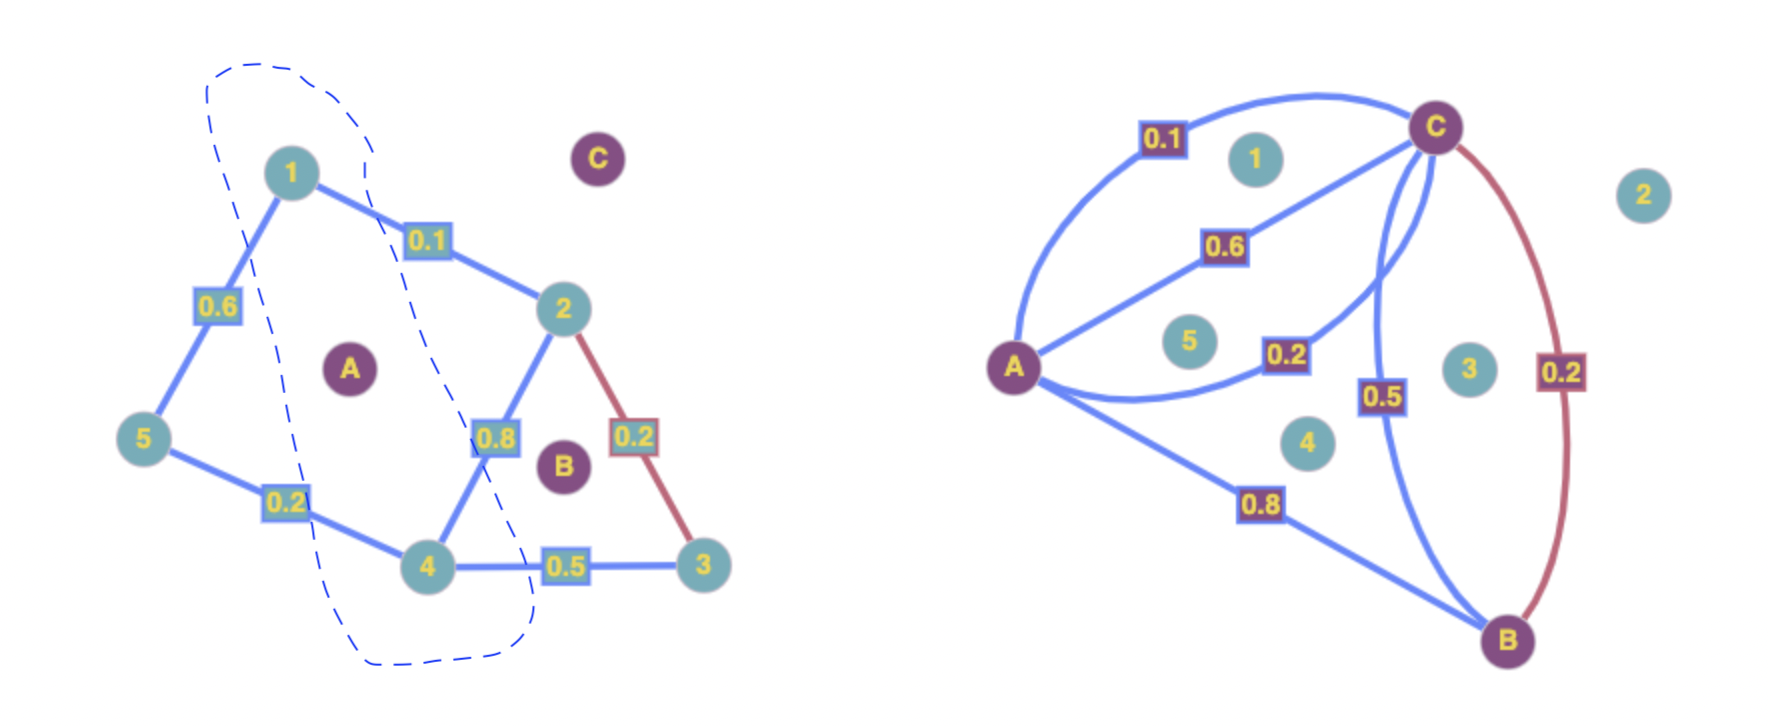
\includegraphics[scale=.35]{geom_dual_cut.png}
    \caption{The minimum odd-circuit cover of $G$ and the minimum odd-vertex pairing of $G_d$ are shown in red, and the maximum cut of $G$ is shown in blue.}
    \label{fig:hadlock_example}
\end{figure}

\par Other researchers have given polynomial-time algorithms for solving the minimum odd-vertex pairing problem.\cite{Hadlock} Since $(G_d)_d = G$ for an embedding of a planar graph $G$, to find the maximum cut of $G$, we need only embed it, run its geometric dual through one of these algorithms, and convert the result by taking the geometric dual once more. Max-cut solutions for non-planar graphs cannot necessarily be found in polynomial time in this manner because they do not necessarily have a unique geometric dual. \\

\newpage

\subsection{Example: Hadlock's Transformation on a Slightly Complicated Planar Graph}

\par For illustration's sake, we will consider the unweighted problem for this example. Consider the graph $G$ and its geometric dual $G_d$ depicted in Figure \ref{fig:slightly_complicated} below.

\begin{figure}[h]
    \centering
    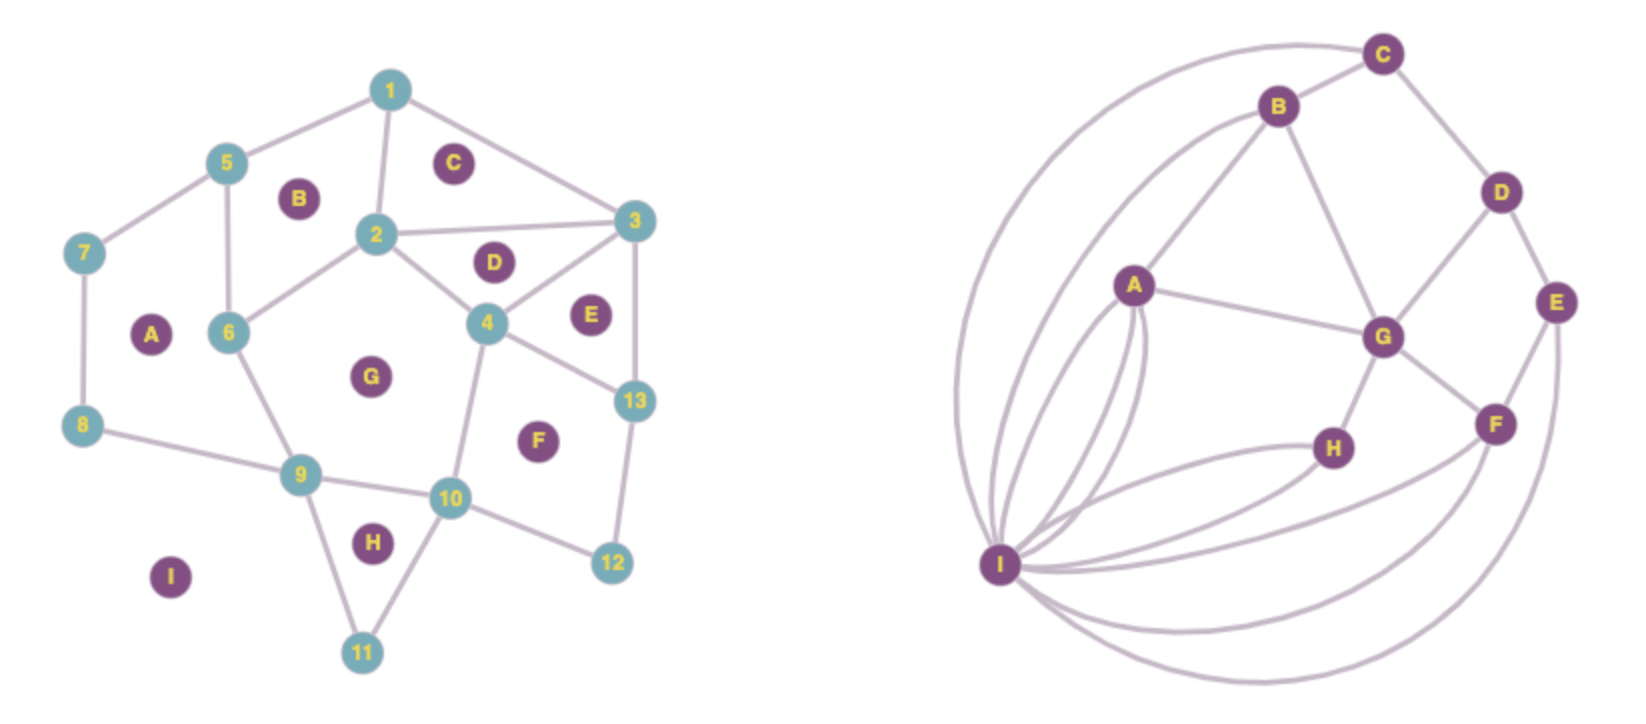
\includegraphics[scale=.35]{planar_dual.png}
    \caption{A planar graph $G$ and its geometric dual $G_d$}
    \label{fig:slightly_complicated}
\end{figure}

\par The vertices of $G_d$ with odd degree are $A$, $C$, $D$, $E$, $G$, and $H$. The reader can confirm visually that the odd-vertex pairing with the fewest edges is $\{(A,B),(B,C),(D,E),(G,H)\}$. This corresponds to the minimum odd-circuit cover in $G$, given by $\{(1,2),(3,4),(5,6),(9,10)\}$. Removing this set of edges indeed eliminates all odd cycles from the graph. And as Figure \ref{fig:slightly_complicated_cut} shows, the complement of this odd-circuit cover is indeed a cut, with a weight of 16. We conclude that this is the maximum cut of $G$.

\begin{figure}[h]
    \centering
    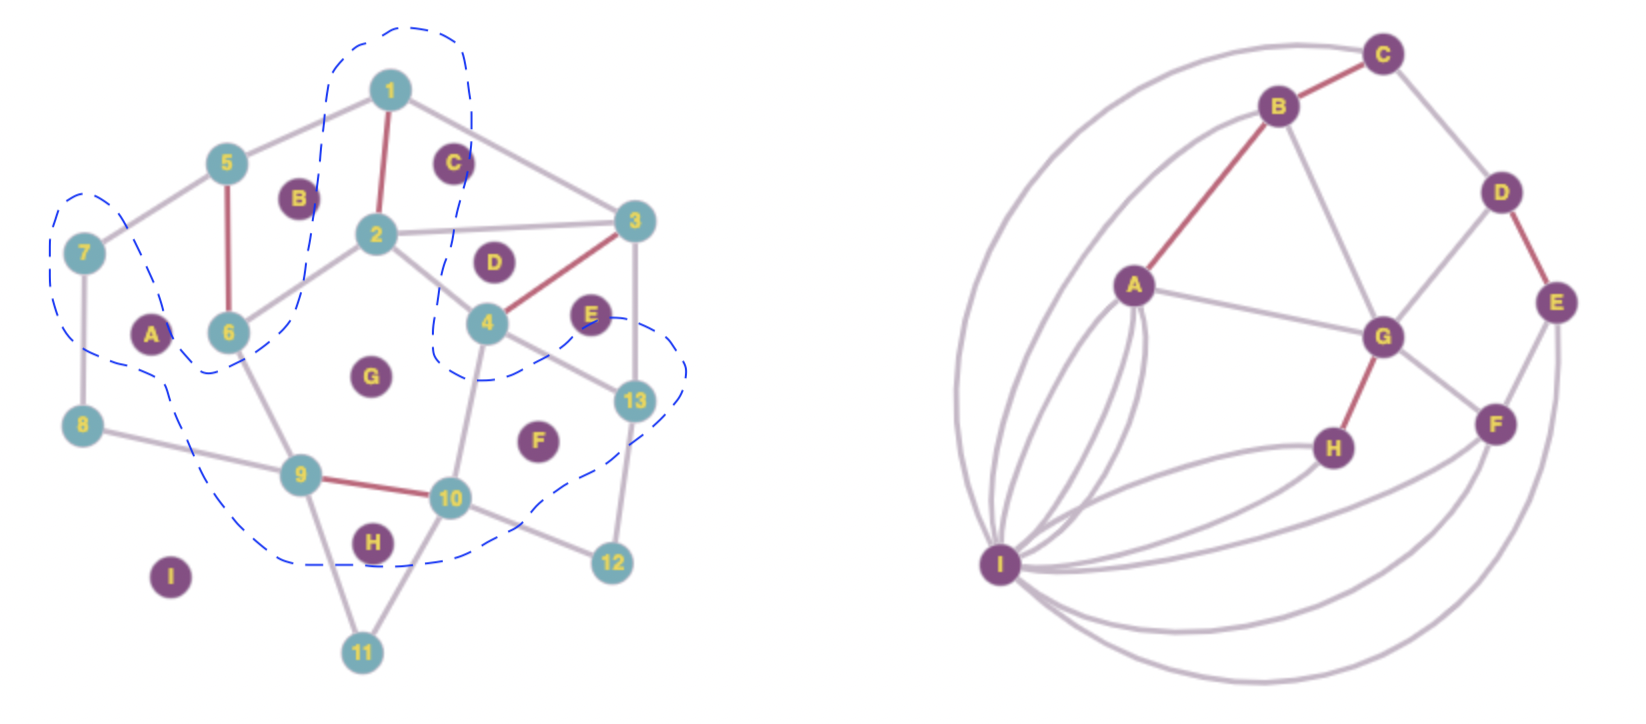
\includegraphics[scale=.35]{planar_dual_cut.png}
    \caption{Using Hadlock's transformation to find the maximum cut of $G$}
    \label{fig:slightly_complicated_cut}
\end{figure}


\section{NP-Approximation: The Goemans-Williamson Relaxation of Max-Cut}

\par In 1995, Goemans and Williamson made a significant breakthrough that has not yet been improved upon. Their algorithm returns a cut with a weight of at least .878 times the weight of the true maximum cut.\cite{GW} \\

\par Recall the function that gives the weight of a cut $(S,\bar{S})$ is $$w(S,\bar{S}) = \frac{1}{2}\sum_{i<j} w_{ij}(1-y_iy_j).$$ Noting that $y_i$ and $y_j$ can be considered unit vectors in $\mathbb{R}^1$, Goemans and Williamson ``relax'' the max-cut problem by swapping out $y_i$ and $y_j$ for unit vectors $\vec{v}_i$ and $\vec{v}_j$ in $\mathbb{R}^n$, where $n$ is the number of vertices in the graph. Maximizing the new objective function $f(x) = \frac{1}{2}\sum_{i<j} w_{ij}(1 - \vec{v}_i \cdot \vec{v}_j)$ is a simpler task because it is a \textit{semi-definite program}.\\

\par Let $X$ be the matrix with $\vec{v}_i$ in the $i$th column, $1 \le i \le n$, and let $Y = X^T X$. Then $Y$ is positive semi-definite, meaning $\vec{v} X^T \vec{v} \ge 0$ for all $\vec{v} \in \mathbb{R}^n$.\cite{GW} Since entry $y_{ij} = \vec{v}_i \cdot \vec{v}_j$, we obtain a new objective function: $$f(x) = \frac{1}{2}\sum_{i<j} w_{ij}(1 - y_{ij}).$$ Let $Z^*$ be the value of this function applied to a solution set of vectors. While the problem of maximizing $Z^*$ is not in $P$, we can pick a small constant $\epsilon > 0$ and find a solution with value $Z^* - \epsilon$ in polynomial time. The upper bound on running time depends only on $n, \epsilon,$ and the sum of the weights $w_{ij}$.\cite{GW} \\

\par After finding the optimal set of vectors using an algorithm for the semi-definite program, randomly select a new vector $\hat{r}$ that passes through the origin of $\mathbb{R}^n$. Then let $S := \{i|v_i\cdot \hat{r} \ge 0\}$. In other words, $\hat{r}$ is normal to a hyperplane in $\mathbb{R}^n$, and all the vectors above the plane are in $S$ while all the vectors below are in $\bar{S}$. As Goemans and Williamson prove, the expected weight of the resulting cut $(S,\bar{S})$ is at least $\alpha(Z^* - \epsilon)$, where $\alpha = min_{0\le \theta \le \pi} \frac{2}{\pi}\frac{\theta}{1-\cos{\theta}} > 0.878$.\cite{GW} \\


\section{Discussion}

\par While the max-cut problem will likely never be shown to be in $P$, the Goemans-Williamson reduction provides a powerful approximation and allows for meaningful analysis of large graphs. Applied repeatedly, it can illuminate even more aspects of a graph; for example, the general diffusion or concentration of weights can be characterized by the average size of an intersection of different cuts returned by the algorithm.\cite{GW} \\

\par Goemans and Williamson also manipulate their procedure to find an approximation for a maximum cut on a directed graph, in which the sign on a weight depends on the order of its vertices (in other words, $w_{ij} = -w_{ji}$). Their approximation produces a solution set with optimal value 0.796. Neural networks are directed non-planar graphs, so this result might be effectively applied to analyzing their architecture. \\

\par Furthermore, max-cut algorithms may prove useful as a part of the neural network itself by inserting them among the neural layers. The difficulty of using such ``combinatorial solvers'' is that their output is discrete, so the output function is piecewise-constant and its derivative is 0 at all points. \\

\par Until recently, this was a prohibitive obstacle to using combinatorial solvers in DNN architecture. DNNs learn using a technique called gradient descent, which depends on the output function of each neuron having a nonzero derivative. However, some researchers showed that the piecewise-constant output function of a combinatorial solver can be interpolated to a continuous function with non-zero derivatives, allowing gradient descent to take place and improve the combinatorial solver.\cite{Vlast} If combinatorial solvers are successfully introduced into DNN architecture, many exciting applications await. 

\begin{thebibliography}{99}
    \bibitem{GW} Goemans, M. X. \& Williamson, D. P. (1995). ``Improved approximation algorithms for maximum cut and satisfiability problems using semidefinite programming.'' In {\em Journal of the ACM} 42(6), 1115–1145. \\
    https://doi.org/10.1145/227683.227684.
    \bibitem{Hadlock} Hadlock, F. (1975). ``Finding a maximum cut of a planar graph in polynomial time.'' In {\em SIAM Journal on Computing} 4(3), 221-5. \\
    https://doi.org/10.1137/0204019.
    \bibitem{Karp} Karp, R. M. (1972). ``Reducibility among Combinatorial Problems.'' In: Miller, R.E., Thatcher, J.W., Bohlinger, J.D. (eds) {\em Complexity of Computer Computations}. The IBM Research Symposia Series. Springer, Boston, MA. \\ https://doi.org/10.1007/978-1-4684-2001-2\_9.
    \bibitem{Shahriari} Shahriari, S. (2022). {\em An Invitation to Combinatorics}. Cambridge University Press, London, UK.
    \bibitem{Vlast} Vlastelica, M., Paulus, A., Musil, V., Martius, G., \& Rolínek, M. (2019). ``Differentiation of Blackbox Combinatorial Solvers.'' \\
    https://doi.org/10.48550/ARXIV.1912.02175.
\end{thebibliography}
\end{document}
